\documentclass[12pt]{article}
%\linespread{1.6}

\usepackage{graphicx}
\usepackage{booktabs}
\usepackage{longtable}
\usepackage{tabu}
\usepackage{listings}
\usepackage{hyperref}
\usepackage{tcolorbox}
%\usepackage{neurips_2019}
\usepackage[utf8]{inputenc}
\usepackage[T1]{fontenc}
\usepackage{url}
\usepackage{amsfonts}
\usepackage{nicefrac}
\usepackage{microtype}

\usepackage{amsmath}
\usepackage{amssymb}
\graphicspath{{images/}}
\usepackage{indentfirst}
\usepackage{lipsum}
\usepackage{xcolor}
\usepackage{soul}
\usepackage{setspace}
\usepackage[
backend=biber,
style=alphabetic,
sorting=ynt
]{biblatex}
\usepackage{hyperref}
\usepackage{tikz}
\usetikzlibrary{shapes.geometric, positioning, fit, arrows.meta}

%-----------some colors
\newcommand{\standardcolor}{blue}
\newcommand{\unlimicolor}{red}
\newcommand{\combcolor}{green}

\tikzstyle{startstop} = [rectangle, rounded corners, 
minimum width=3cm, 
minimum height=1cm,
text centered, 
draw=black, 
fill=\standardcolor!30]

\tikzstyle{combFn} = [trapezium, 
trapezium stretches=true, % A later addition
trapezium left angle=70, 
trapezium right angle=110, 
minimum width=3cm, 
minimum height=1cm, text centered, 
draw=black, fill=\combcolor!50,
rounded corners]

\tikzstyle{unlimiFn} = [trapezium, 
trapezium stretches=true, % A later addition
trapezium left angle=70, 
trapezium right angle=110, 
minimum width=3cm, 
minimum height=1cm, text centered, 
draw=black, fill=\unlimicolor!50,
rounded corners]

\tikzstyle{standardFn} = [trapezium, 
trapezium stretches=true, % A later addition
trapezium left angle=70, 
trapezium right angle=110, 
minimum width=3cm, 
minimum height=1cm, text centered, 
draw=black, fill=\standardcolor!50,
rounded corners]

\tikzstyle{process} = [rectangle, 
minimum width=3cm, 
minimum height=1cm, 
text centered, 
text width=3cm, 
draw=black, 
fill=orange!30]
\tikzstyle{decision} = [ellipse, rounded corners,
minimum width=3cm, 
minimum height=1cm, 
text centered, 
draw=black, 
fill=\standardcolor!30]
\tikzstyle{arrow} = [thick,->,>=stealth]
%\usepackage{endfloat}
\addbibresource{sections/references.bib}
\singlespacing
\addtolength{\oddsidemargin}{-.5in}
\addtolength{\evensidemargin}{-.5in}
\addtolength{\textwidth}{1in}

\addtolength{\topmargin}{-.5in}
\addtolength{\textheight}{1in}

\DeclareMathOperator{\softmax}{softmax}
%-----------------------------------------------------------

\begin{document}
%\begin{titlepage}
\begin{center}
\large
\textbf{Project Proposal}\\
\Large
\textbf{Long Document Summarization:}\\
\textbf{Augmenting Unlimiformer with Knowledge Graphs\footnote{\today}}\\
\begin{table}[h]
    \centering
    \begin{tabular}{ccc}
        Patrick O'Callaghan&  Sheel Sansare& Tristan Wang\\
         (patocal)& (ssansa2)  & (aawang99)\\
    \end{tabular}
%    \caption{Caption}
    \label{tab:my_label}
\end{table}
\end{center}
%\end{titlepage}

%\section*{Summary}
Place summary here.
\section{Extracting Knowledge Graphs from Long Documents}
\subsection*{REBEL}
We chose REBEL because it is end-to-end (it finds entities and relations at the same time), open-source, and easy to implement using Hugging Face. Also, according to the DocRED paper by Yao et al \cite{yao2019DocRED}, pretrained REBEL yields the best joint entity and relation extraction (NER and RE) result compared with the benchmark among all models sampled, with a relation F1 score of 47.1\footnote{https://paperswithcode.com/sota/joint-entity-and-relation-extraction-on-3}.

Since the pre-trained REBEL model has a token limit, we chose to split the LD into 128-token chunks before extracting head-relation-tail triplets from each chunk. Next, we used NetworkX to assemble the triplets and form a directed KG. The code for our REBEL implementation can be found here\footnote{https://github.com/patrickocal/unlimiformer/blob/main/rebel.py}.

**Why 128 span length?**

**Why extract triplets (and not extract triplets typed)?**
\subsection*{DyGIE++} Another relation extraction method we explored for
building KGs is DyGIE++ which refines and scores text spans designed to capture
both intra-sentence and cross-sentence context. We have cloned the code from
the official GitHub repository (\url{https://github.com/dwadden/dygiepp}) and
attempted to replicate the process of training a model for relation extraction
on the SciERC dataset, but have not yet been successful due to technical
difficulties. To resolve this issue, we aim to raise a GitHub issue and
continue to debug as needed, in anticipation that DyGIE++ may be used later on
in our project.

\subsection*{LlamaIndex}
\texttt{LlamaIndex} is a framework for connecting data sources for
Large-Language Models. In particular \texttt{LlamaIndex} has a class called
\texttt{KnowledgeGraphIndex}. We have established that the latter is compatible
with \texttt{FAISS} which is the datastore that \texttt{unlimiformer} uses to
conduct a $k$-nearest neighbor search of top-level hidden state encodings that
are most relevant to the query.
\url{https://github.com/run-llama/llama_index/issues/8767}.
This means that we can store the Knowledge Graph we create using LlamaIndex as
a FAISS datastore. The idea is to create a secondary channel for the attention
mechanism. The potential advantage is characterised in the following notebook:
\href{https://github.com/run-llama/llama_index/blob/main/docs/examples/index_structs/knowledge_graph/KnowledgeGraphIndex_vs_VectorStoreIndex_vs_CustomIndex_combined.ipynb}{KG-datastore-notebook}.
If a nearest neighbor search over a KG produces fewer, but more relevant
results, this may help focus the cross-attention mechanism on what is most
important (see figure \ref{fig-kg-datastore-example}).


\section{Understanding and Implementing Unlimiformer}
Unlimiformer \cite{bertsch2023unlimiformer} is a nontrivial way to augment
Large-Language Models. It involves capturing hidden states from the encoder and
placing them in a datastore. We have successfully run basic
\texttt{inference\_example.py} for our baseline \texttt{unlimiformer} model. We
have also successfully trained the baseline Bart model on the GovReport
dataset. We report our initial results in section \ref{sec-training-appendix}.
We encountered a number of issues during this step and we raised Github issues
with the authors/developers of \texttt{unlimiformer} (see
\url{https://github.com/abertsch72/unlimiformer/issues/33}).

We have also taken significant steps towards understanding the
\texttt{unlimiformer} methodology and codebase. We are in detailed discussions
with the authors in this respect (see
\url{https://github.com/abertsch72/unlimiformer/issues/55}). We have made
detailed comments to the codebase to make it more readable and understandable
to ourselves and others (see documents with ``rich comments'' updates in the
forked repository
\url{https://github.com/patrickocal/unlimiformer/tree/main/src})

The goal is to be able to suitable modify and augment the \texttt{unlimiformer}
codebase with Knowledge Graphs. We have learnt that \texttt{unlimiformer} only
uses the FAISS datastore for inference at the testing stage. Thus, if we are to
create a secondary FAISS datastore (using the fact that a LlamaIndex
KnowledgeGraphIndex can be stored as using FAISS), then the same applies. This
presents a potential opportunity for us in that we may be able to replace FAISS
and the \texttt{faiss.knn\_gpu} method with related PyG methods such as 
\texttt{pool.knn\_graph} which would potentially allow us to extract relations
from the $k$-nearest entities. This presumes we are able to establish and
implement an isomorphism between entities and bags of tokens. \emph{***We would
  appreciate staff feedback and a discussion/meeting in relation to whether we
  should pursue this or whether we should pursue other less technical
approaches to integrate KGs with the unlimiformer approach.***} 

We discuss these in the next section.


\section{Next Steps}

One next step would be
fine-tuning the REBEL model on the long-document summarization datasets we
chose, namely the Hugging Face versions of GovReport \cite{huang2021efficient} 
and BookSum \cite{kryscinski2021booksum}. The REBEL model is proven to be
relatively flexible, having been fine-tuned on at least 4 widely-used relation
extraction (RE) datasets of diverse contexts (CONLL04, DocRED, NYT, and ADE)
and performed well on most of them. However, we bear in mind that the 4
aforementioned datasets differ significantly from the one we propose. DocRED
and ADE entities are words or short phrases, while CONLL04 and NYT entities are
sentences from news articles. On the other hand, the entities in our dataset
will be summaries. Fortunately, DocRED benchmark data 
\url{https://paperswithcode.com/sota/joint-entity-and-relation-extraction-on-3}
suggests that, when pre-trained, REBEL performs well on joint entity and
relation extraction on DocRED, which is similar to what we are trying to
accomplish.

As such, we plan to train REBEL on GovReport and BookSum using the method
outlined in part 4 of the original REBEL paper
\cite{huguet2021rebel}. We note that even though REBEL
as a standalone model can extract more than 200 different relation types, this
may still prove insufficient for summarizing long documents. Should this be the
case, we plan to implement a 2-stage extraction process. One such option would
be to use DyGIE for the entity extraction, then use DREEAM for the relation
extraction.

Our long-document summarization project is dependent on the fact that KGs can
encode the key semantic relationships between entities in a document in a more
concise manner than a full datastore of the entire long document. We aim to
evaluate the quality of our KGs by feeding them into a language model to obtain
a hidden encoding of the the KG. Then, we will evaluate them against the gold
summaries provided in the GovReport and BookSum datasets using ROUGE-1
(unigram), ROUGE-2 (bigram), ROUGE-L (sub-sequence), and BERTScore. The ROUGE
metrics compare summarization via lexical overlap between the model-generated
and gold summaries, while BERTScore compares the semantic similarities of the
two using the BERT embeddings. 

If the KGs produced by REBEL are too large to be converted directly into
summaries, we will use the graph-to-graph (G2G) method detailed in part 6.2 of
\cite{wu2020extracting}. In short, the G2G method encodes the input KG with a
GAT and uses the resulting node representations to make a binary salience
prediction and generate a summary subgraph. We can then feed this smaller
subgraph into ChatGPT and obtain a summary.

\newpage
\printbibliography
\appendix
\newpage
\section{Example of Extracted Knowledge Graph}
\begin{figure}[hp]
    \centering
    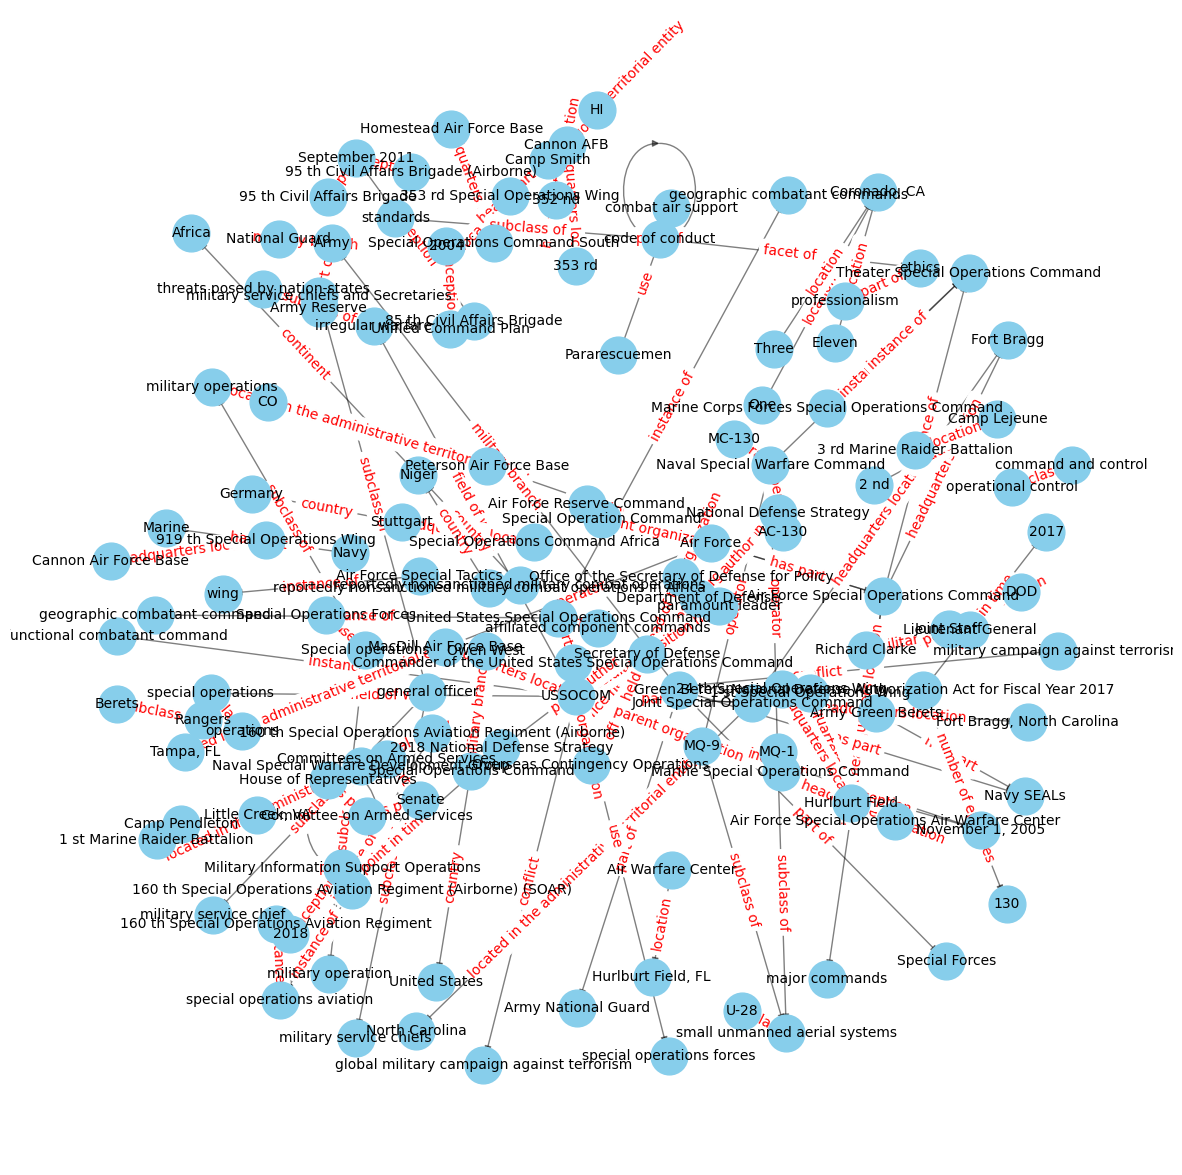
\includegraphics[width=14cm]{images/KG.png}
    \caption{KG for the first document of the GovReport validation set:
    extracted using REBEL. Node labels are in black and edge labels are in red.}
    \label{fig-galaxy}
\end{figure}

\newpage
\section{KG-Datastore Example}
\begin{figure}[h]
  \centering
  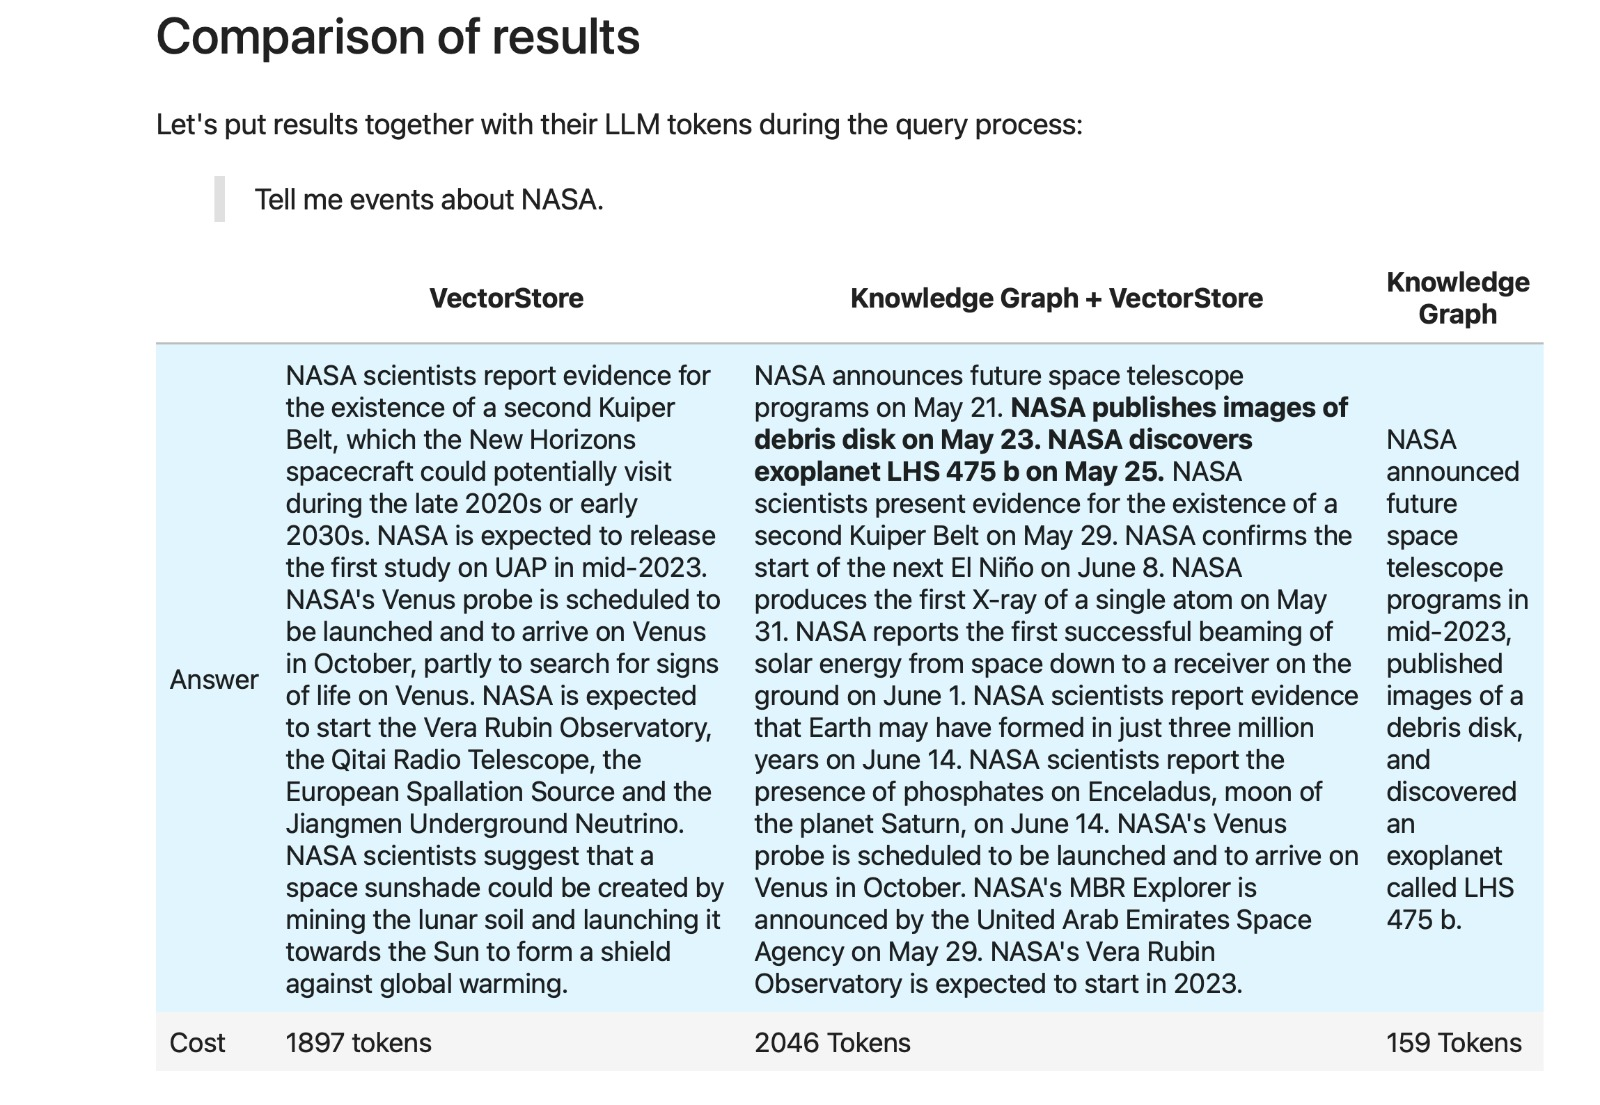
\includegraphics[width=16cm]{images/kg-datastore-example.jpeg}
  \caption{This is an example taken from
  \href{https://github.com/run-llama/llama_index/blob/main/docs/examples/index_structs/knowledge_graph/KnowledgeGraphIndex_vs_VectorStoreIndex_vs_CustomIndex_combined.ipynb}{KG-datastore-notebook}
that shows how the different structure of a Knowledge graph produces very
different results in the associated, yet different, context of querying a
document or collection of documents.}
  \label{fig-kg-datastore-example}
\end{figure}


\newpage
\section{Training Bart on GovReport using Unlimiformer}
\label{sec-training-appendix}

\begin{figure}[!htb]
\minipage{0.49\textwidth}
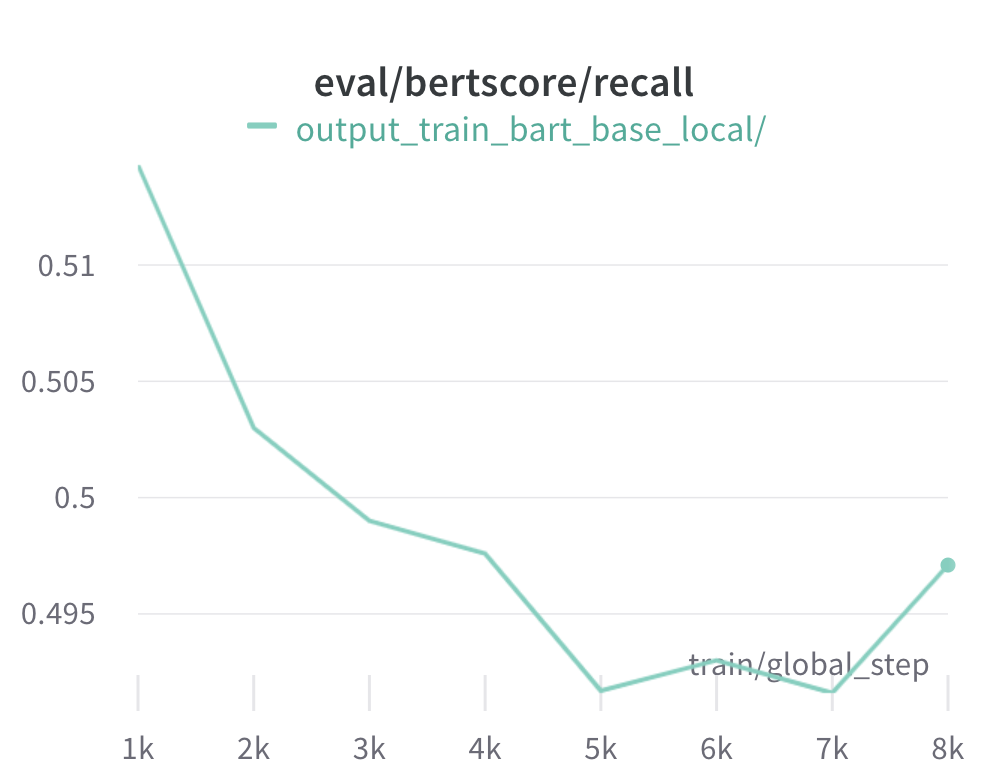
\includegraphics[width=\linewidth]{wandb/charts/Section-2-Panel-0-5gq0m8uvz}
\caption{}
\endminipage\hfill
\minipage{0.49\textwidth}
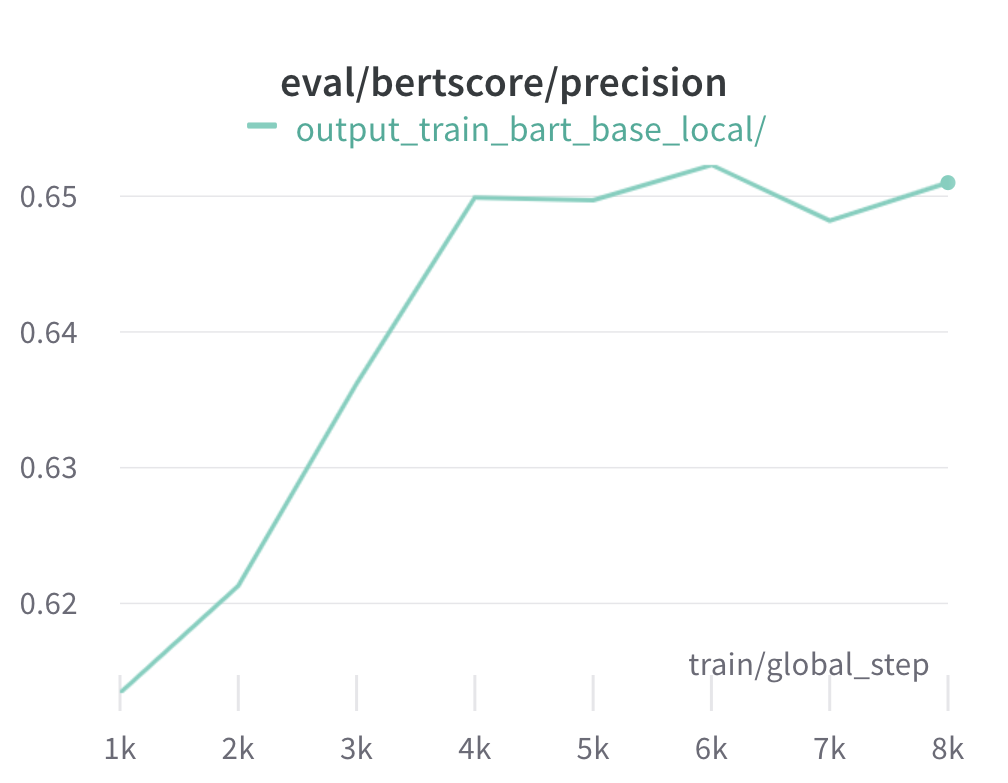
\includegraphics[width=\linewidth]{wandb/charts/Section-2-Panel-1-omp5lgv1w}
\caption{}
\endminipage
\end{figure}

\begin{figure}[!htb]
\minipage{0.49\textwidth}
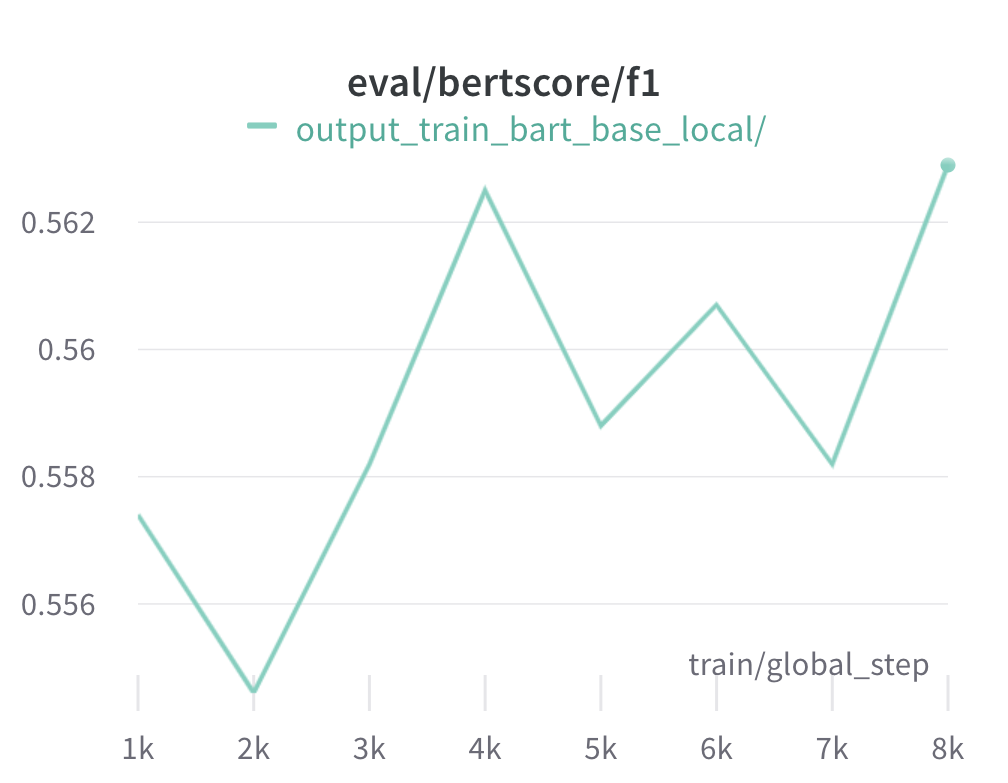
\includegraphics[width=\linewidth]{wandb/charts/Section-2-Panel-2-n99sw9rfp}
\caption{}
\endminipage
\end{figure}

\begin{figure}[!htb]
\minipage{0.49\textwidth}
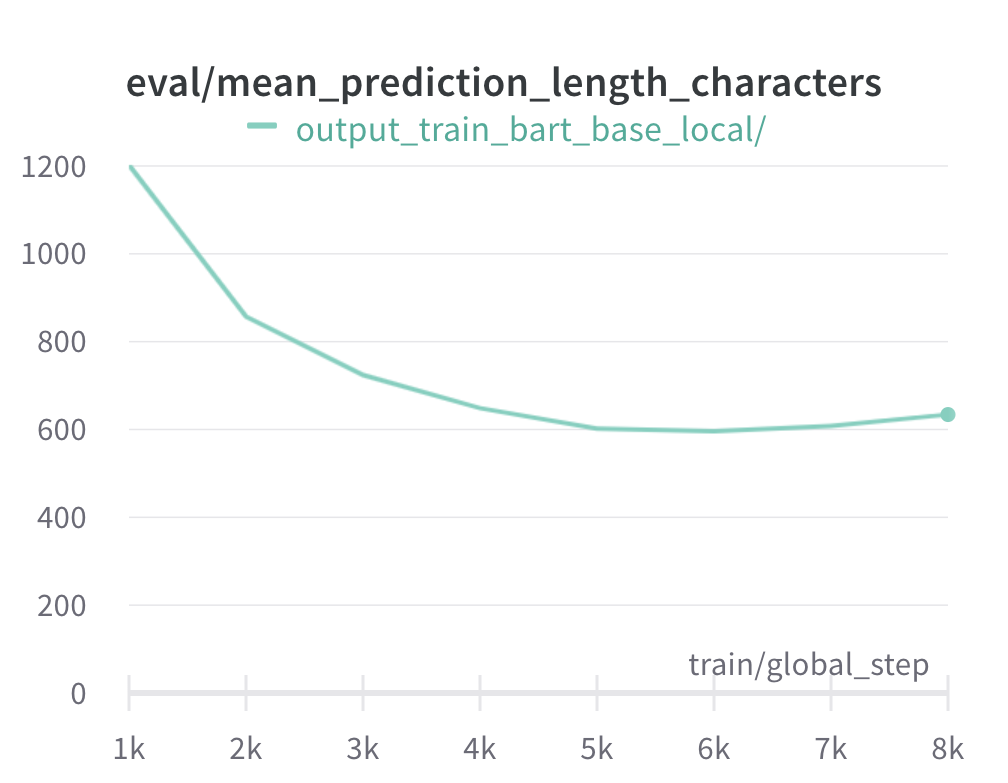
\includegraphics[width=\linewidth]{wandb/charts/Section-4-Panel-0-mbqkjnm1l}
\caption{}
\endminipage\hfill
\minipage{0.49\textwidth}
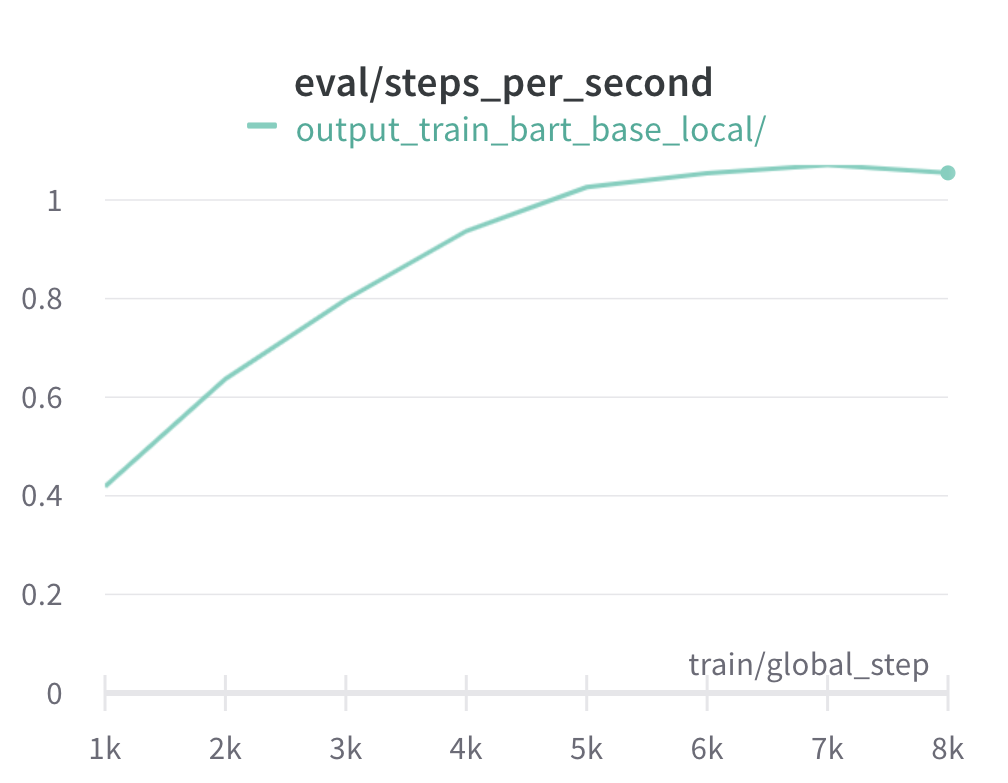
\includegraphics[width=\linewidth]{wandb/charts/Section-4-Panel-1-rouuz3suq}
\caption{}
\endminipage
\end{figure}

\begin{figure}[!htb]
\minipage{0.49\textwidth}
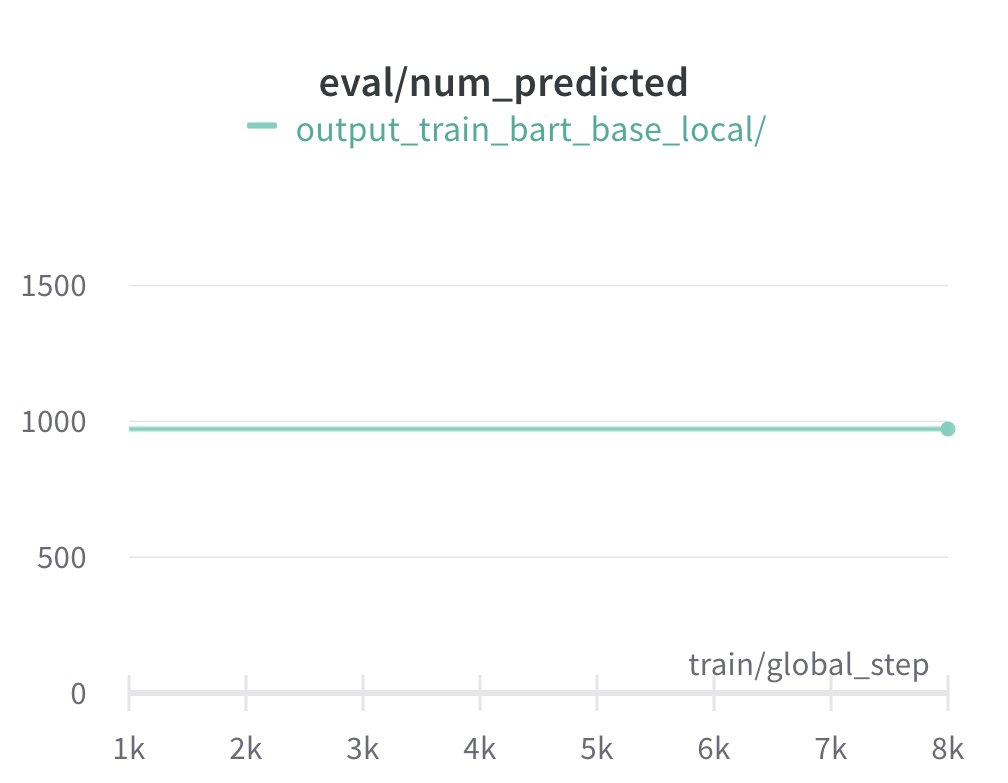
\includegraphics[width=\linewidth]{wandb/charts/Section-4-Panel-2-7v9p2n6qw}
\caption{}
\endminipage\hfill
\minipage{0.49\textwidth}
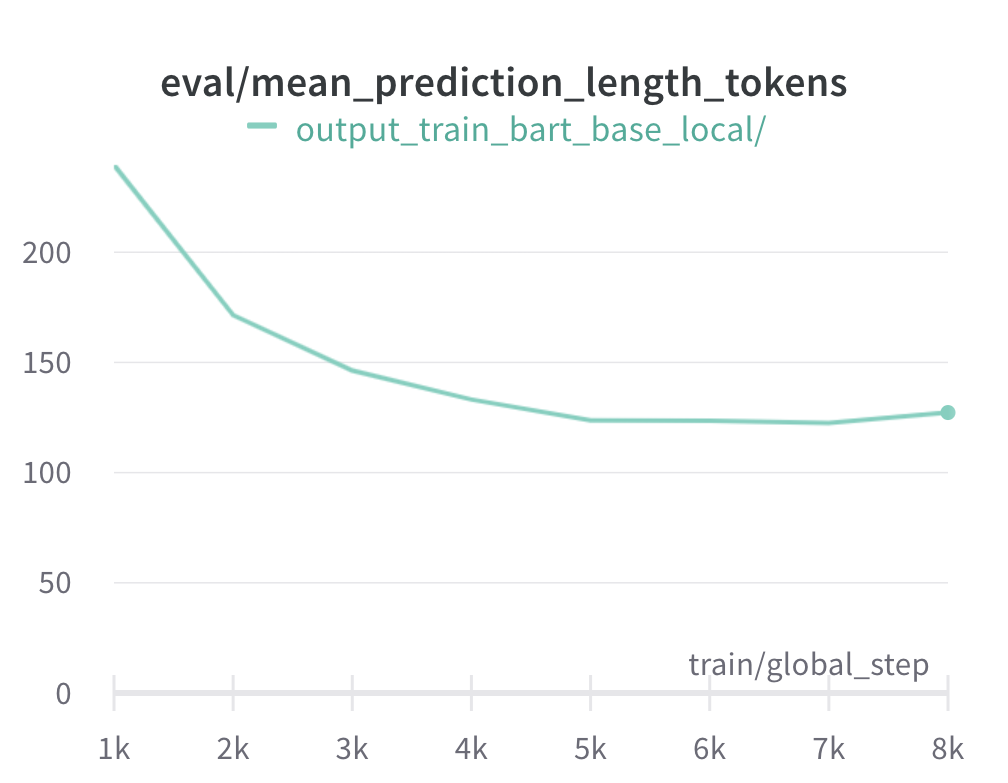
\includegraphics[width=\linewidth]{wandb/charts/Section-4-Panel-3-d4b23g8ks}
\caption{}
\endminipage
\end{figure}

\begin{figure}[!htb]
\minipage{0.49\textwidth}
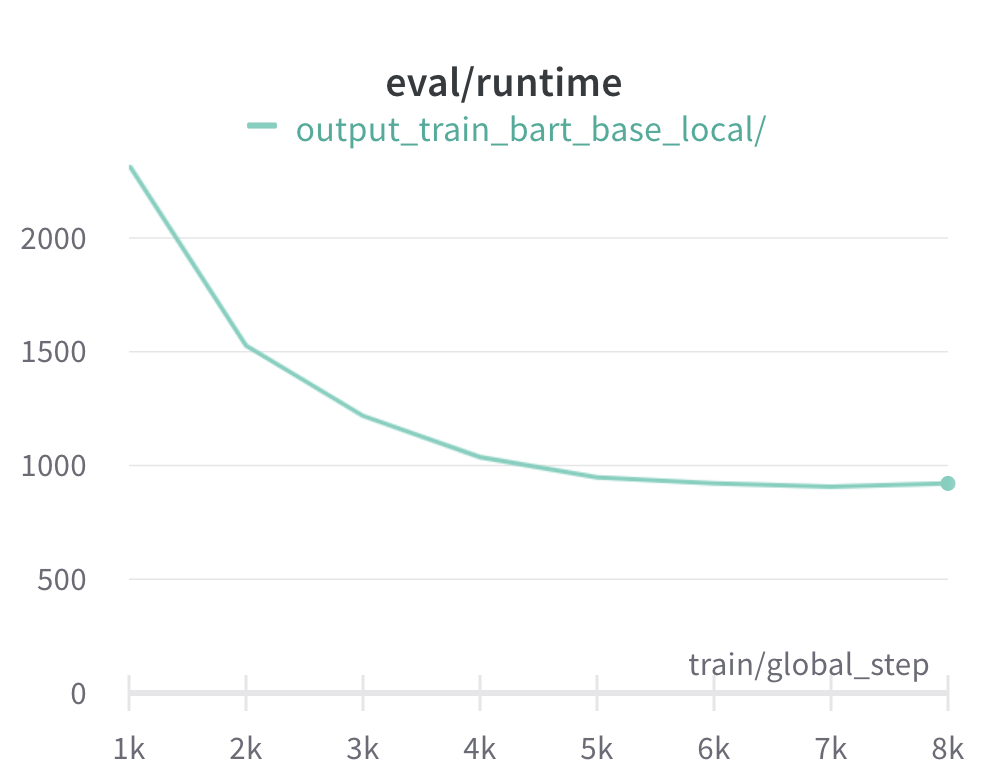
\includegraphics[width=\linewidth]{wandb/charts/Section-4-Panel-4-nuos3yp7v}
\caption{}
\endminipage\hfill
\minipage{0.49\textwidth}
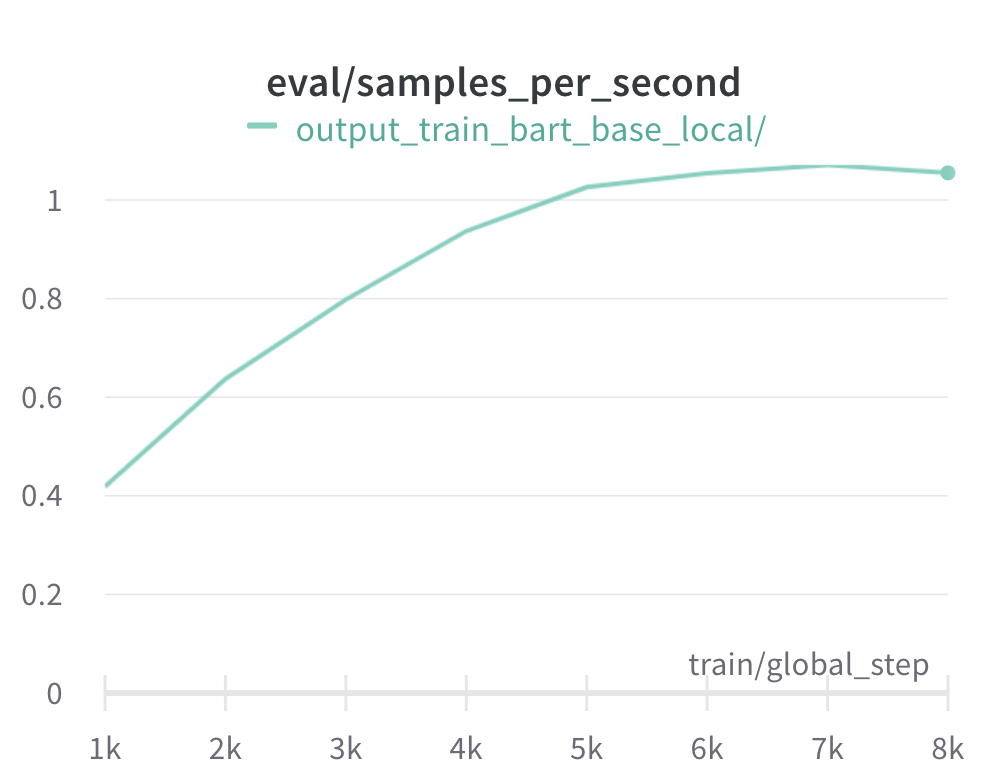
\includegraphics[width=\linewidth]{wandb/charts/Section-4-Panel-5-noz0rp558}
\caption{}
\endminipage
\end{figure}

\begin{figure}[!htb]
\minipage{0.49\textwidth}
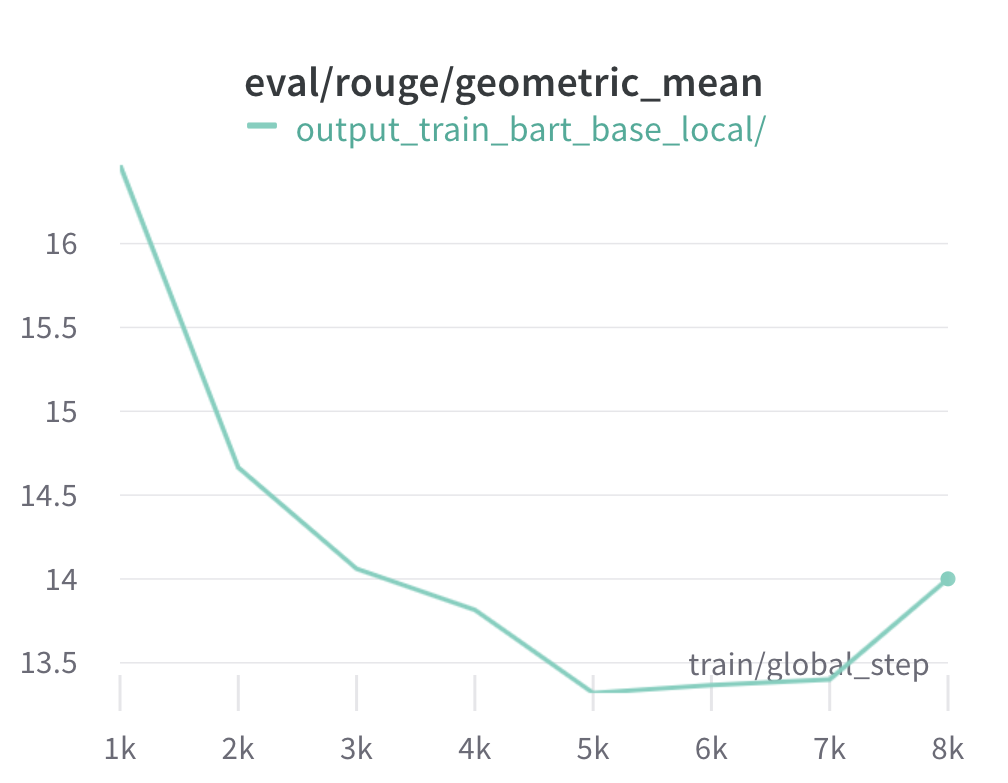
\includegraphics[width=\linewidth]{wandb/charts/Section-6-Panel-0-5w7pojrrj}
\caption{}
\endminipage\hfill
\minipage{0.49\textwidth}
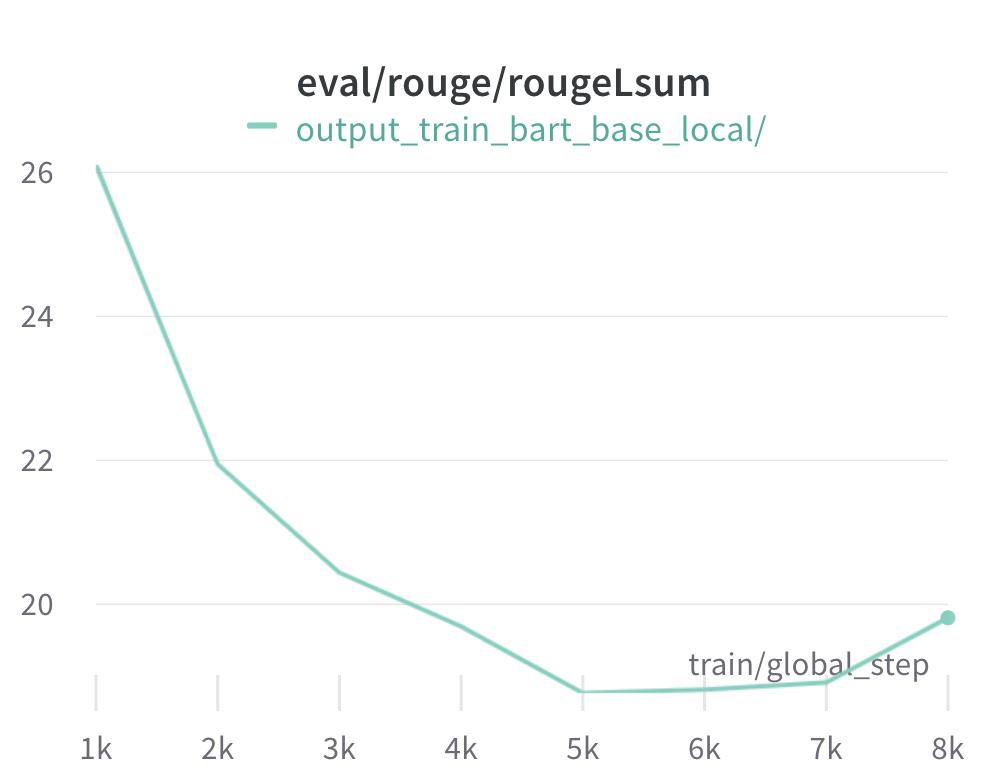
\includegraphics[width=\linewidth]{wandb/charts/Section-6-Panel-1-u7oototqm}
\caption{}
\endminipage
\end{figure}

\begin{figure}[!htb]
\minipage{0.49\textwidth}
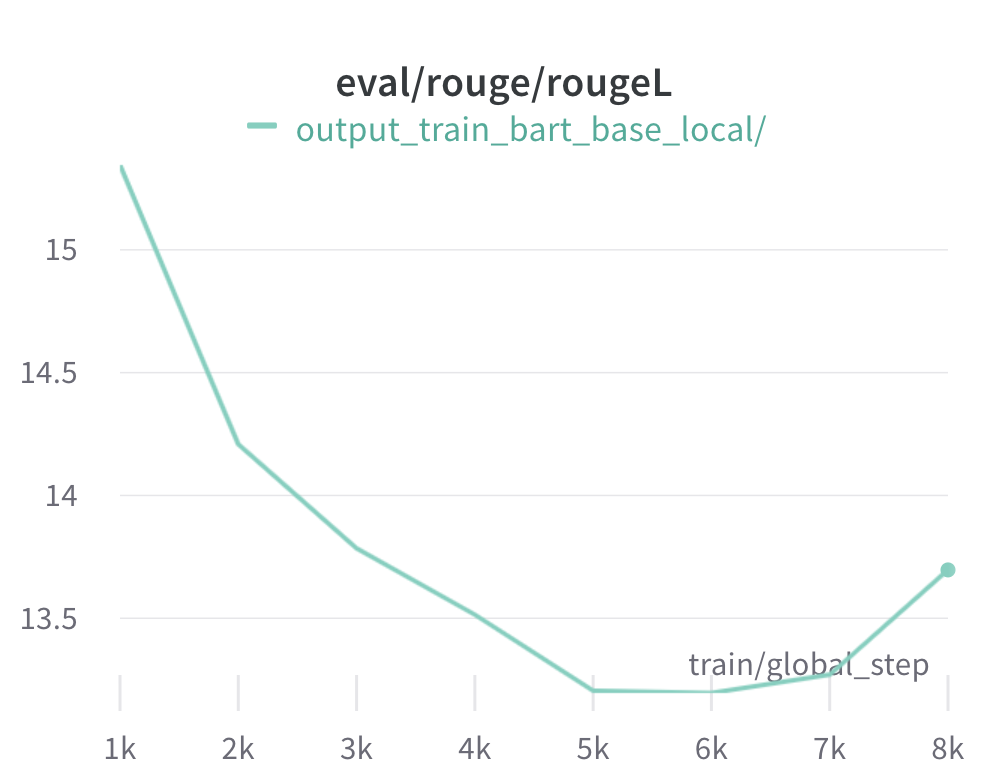
\includegraphics[width=\linewidth]{wandb/charts/Section-6-Panel-2-58cklx5fa}
\caption{}
\endminipage\hfill
\minipage{0.49\textwidth}
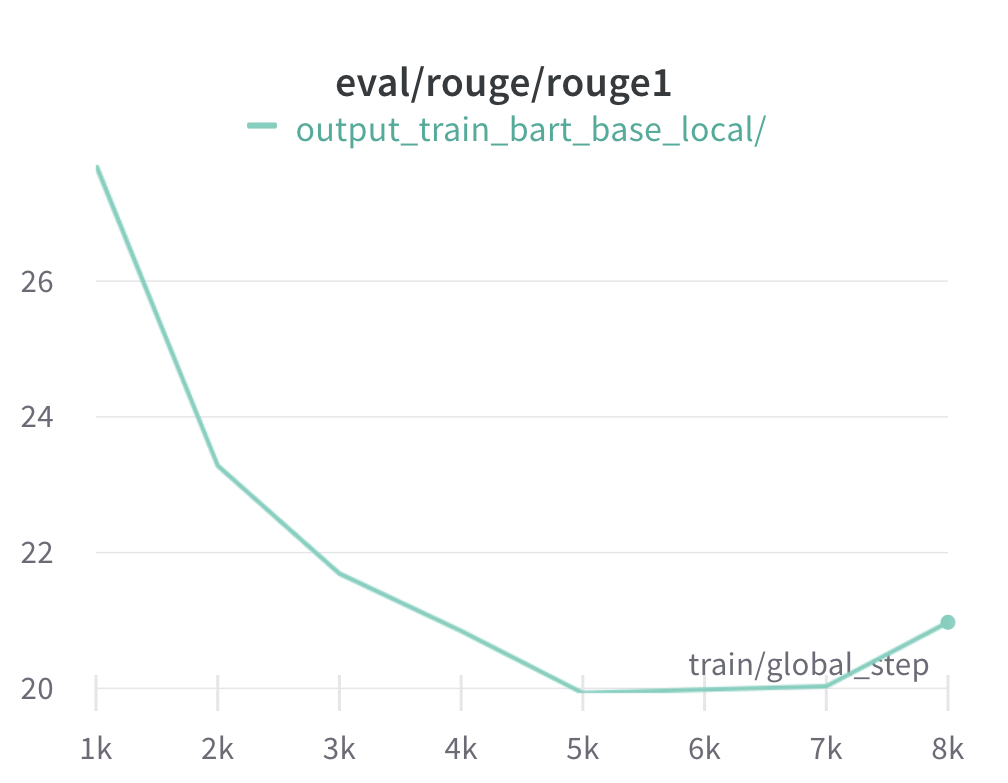
\includegraphics[width=\linewidth]{wandb/charts/Section-6-Panel-3-mu3n5ufdz}
\caption{}
\endminipage
\end{figure}

\begin{figure}[!htb]
\minipage{0.49\textwidth}
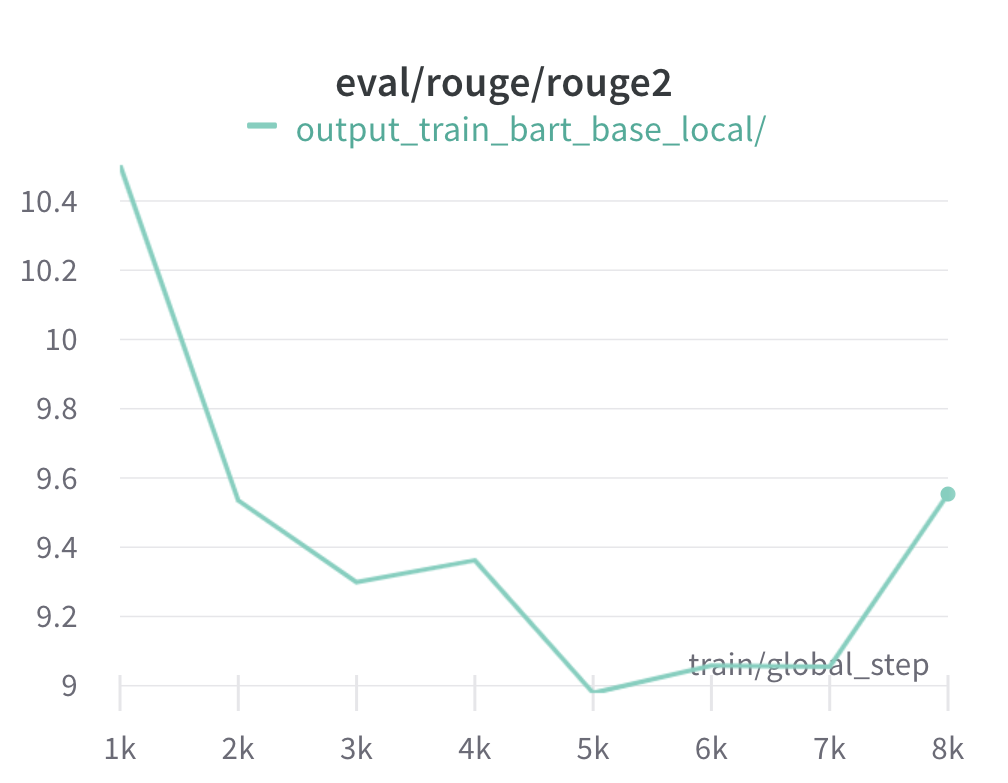
\includegraphics[width=\linewidth]{wandb/charts/Section-6-Panel-4-a7t98duha}
\caption{}
\endminipage
\end{figure}

\begin{figure}[!htb]
\minipage{0.49\textwidth}
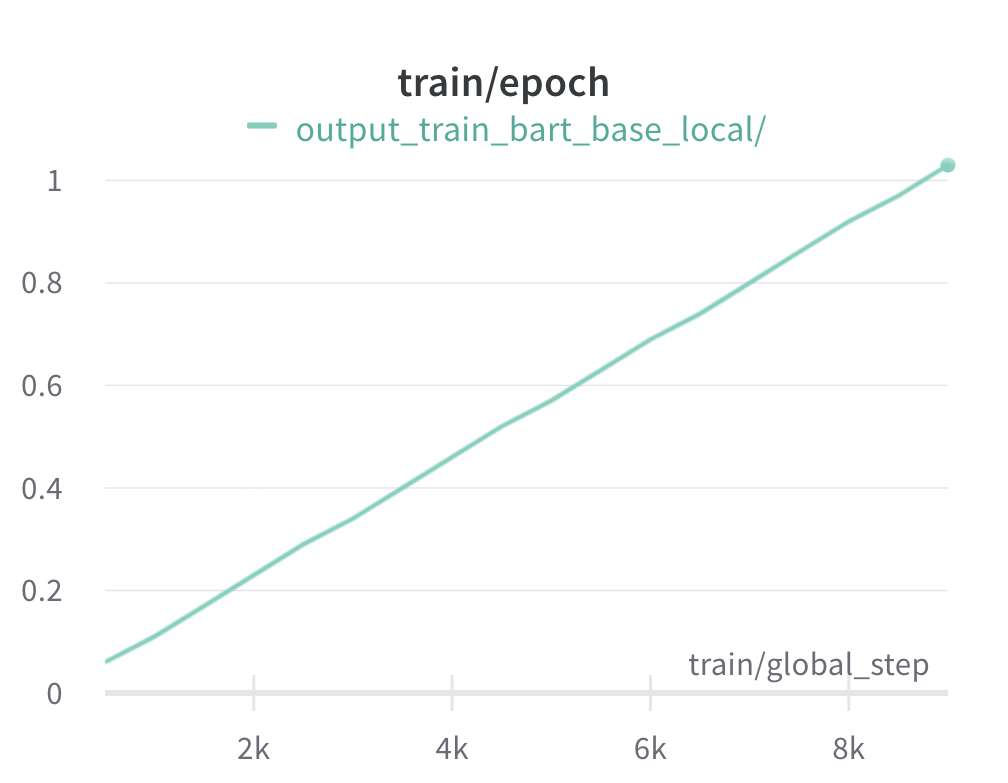
\includegraphics[width=\linewidth]{wandb/charts/Section-8-Panel-0-b9jdvbp9c}
\caption{}
\endminipage\hfill
\minipage{0.49\textwidth}
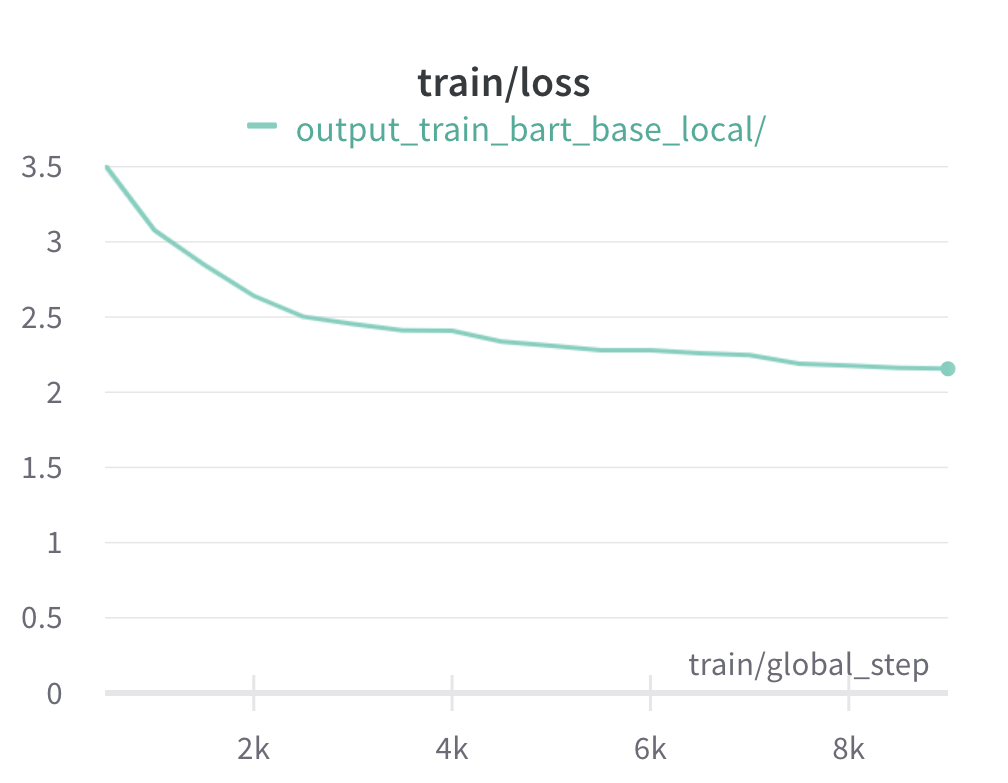
\includegraphics[width=\linewidth]{wandb/charts/Section-8-Panel-1-uc1nwfci0}
\caption{}
\endminipage
\end{figure}

\begin{figure}[!htb]
\minipage{0.49\textwidth}
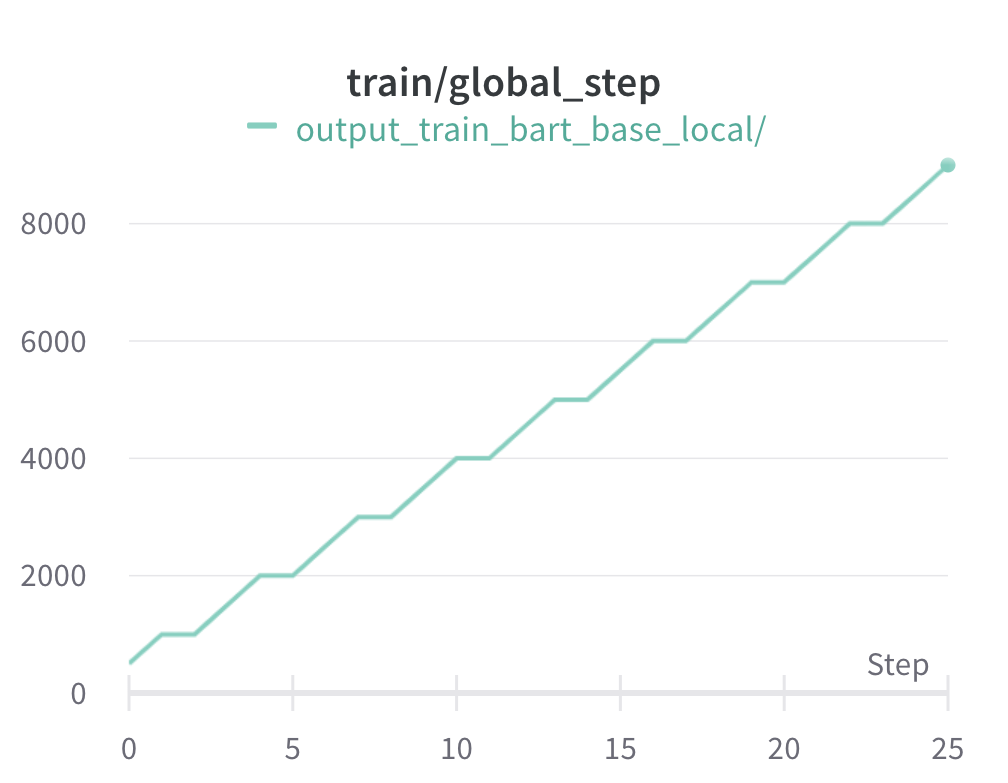
\includegraphics[width=\linewidth]{wandb/charts/Section-8-Panel-2-utzp1vfip}
\caption{}
\endminipage\hfill
\minipage{0.49\textwidth}
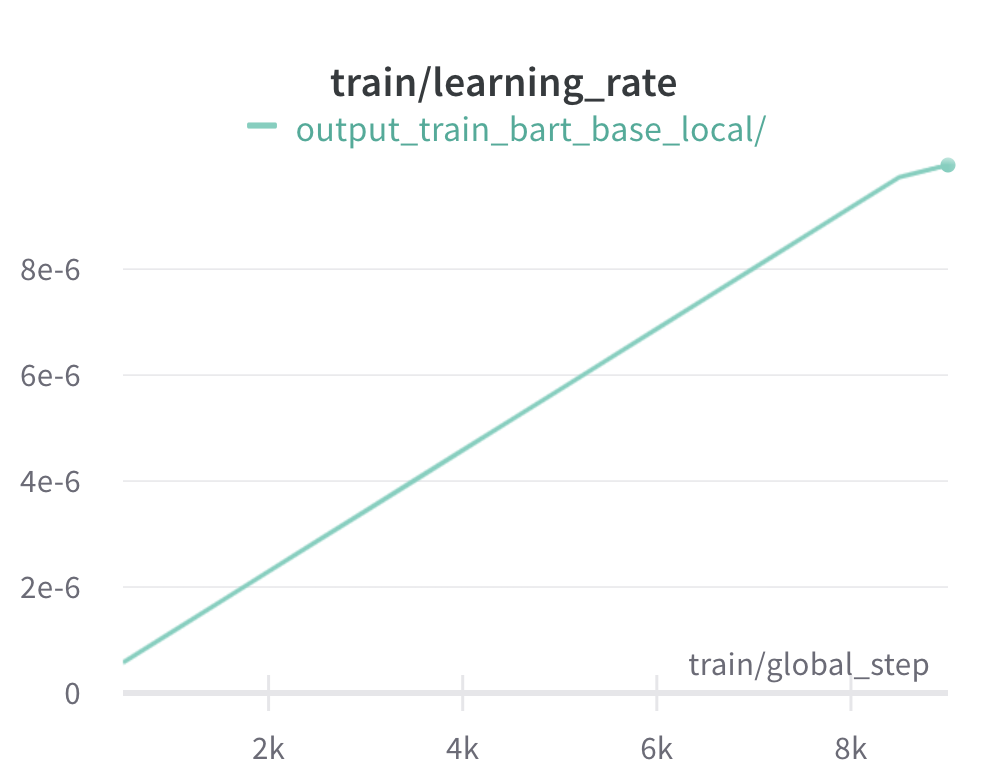
\includegraphics[width=\linewidth]{wandb/charts/Section-8-Panel-3-g06yu99wh}
\caption{}
\endminipage
\end{figure}



\newpage
\end{document}
